\documentclass[conference]{IEEEtran}

\usepackage[T1]{fontenc}
\usepackage[utf8]{inputenc}
\usepackage{cite}
\usepackage{url}
\usepackage{booktabs}
\usepackage{array}
\usepackage{tikz}
\usetikzlibrary{arrows.meta, positioning, shapes.geometric, shapes.misc}

\title{AI-Enabled Social Media Content Generation and Scheduling: An IEEE-Style Research Paper}

\author{
\IEEEauthorblockN{Abhi}
\IEEEauthorblockA{
Department of Computer Science and Engineering\\
Project: AI Social Media Automation Agent
}
}

\begin{document}

\maketitle

\begin{abstract}
Teams that handle social media for small products or services often spend more time moving between drafting, saving, and scheduling tools than actually refining the message they want to publish. This paper examines a working AI-enabled social media automation agent built to simplify that flow. The system combines caption generation, authenticated access, post-history storage, and time-based scheduling inside one web application. Its current implementation uses a React frontend, a FastAPI backend, MongoDB Atlas, JSON Web Token authentication, GPT-4o-mini for text generation, and a Python worker that monitors scheduled posts and updates execution status. The paper focuses on the implemented behavior of the prototype rather than on a purely conceptual framework. In particular, it discusses practical limits already visible in the codebase, including simulated posting paths, timezone interpretation, and credential-handling choices. The project suggests that generative AI can reduce routine drafting effort while still keeping topic selection, review, and scheduling decisions under user control.
\end{abstract}

\begin{IEEEkeywords}
Generative AI, social media automation, FastAPI, React, MongoDB, large language models, content scheduling, digital marketing.
\end{IEEEkeywords}

\section{Introduction}

Generative artificial intelligence is already influencing digital marketing, especially in tasks that involve repeated short-form writing such as captions, hashtags, and campaign variations. Even so, writing support alone is not enough for a usable system. A practical application must also handle login, ownership of generated material, storage of earlier outputs, scheduling, and some form of operational traceability. Recent marketing research supports the productivity gains of GenAI, but it also warns that reliability, review, and brand control remain important when such systems are used in live communication settings \cite{grewal2025,cillo2025}.

The project examined in this paper was built as a lightweight social media assistant rather than as a broad enterprise platform. In its current form, a user can create an account, log in, request an Instagram-style caption and hashtag set for a topic, review previously generated posts, and schedule content for later release. The frontend is implemented as a React single-page interface. The backend uses FastAPI, MongoDB Atlas collections, bcrypt-based password hashing, and JWT bearer authentication. Text generation is handled through GPT-4o-mini. A separate Python worker checks pending scheduled posts every ten seconds and marks due entries as posted.

What makes the project worth documenting is not novelty at the model level, but the way common web engineering decisions shape the actual behavior of a GenAI tool. The present implementation already reveals useful design lessons: generated posts are tied to individual users, scheduled items are persisted separately from generated drafts, and posting is simulated rather than connected to live social APIs. The paper therefore contributes a grounded case study of how a small full-stack GenAI application behaves in practice, where its boundaries appear, and what would need to change before it could move from demonstration use to a more production-ready workflow.

\section{Literature Review}

Research on generative AI in marketing has expanded quickly, but much of it still discusses strategic potential more than the everyday design of small working systems. Grewal et al. describe GenAI as influential across communication, service, and content creation, while also stressing that oversight and governance remain necessary \cite{grewal2025}. Cillo and Rubera make a related point from the innovation side: the real value of these tools depends on how organizations reshape their processes around them rather than simply inserting a model into an old workflow \cite{cillo2025}. That point matters here because a social media assistant is only useful when generation, storage, review, and scheduling are connected in a manageable way.

The literature also suggests where systems like this one could develop next. Chen et al. describe personalization as moving toward more interactive and adaptive LLM-based behavior \cite{chen2024}. In a project such as this, that would mean going beyond a plain topic prompt and incorporating tone, platform, audience, and campaign intent. Krugmann and Hartmann further show that generative models are changing sentiment analysis itself \cite{krugmann2024}, which opens the door to a workflow in which the system not only drafts a caption but also helps evaluate whether that caption fits the intended communication style.

At the same time, the current literature offers enough caution to prevent overclaiming. General surveys of large language models still point to prompt sensitivity, uneven factual reliability, and unresolved evaluation challenges \cite{kumar2024llm}. Studies on creativity and co-creation are encouraging, but they mostly support the idea of collaborative use rather than replacement of human judgment \cite{hubert2024,mcguire2024}. Work on social judgment, misinformation, and broader public effects shows why fluency alone cannot be treated as trustworthiness \cite{mittelstadt2024,govindankutty2024,kudina2025}. For that reason, the present paper frames the prototype as a user-assisted drafting and scheduling system whose value depends on keeping a human decision point in the loop.

\section{Proposed System}

The proposed system is a web-based AI assistant for generating and scheduling social media content. A user authenticates through the frontend, receives a JWT token from the backend, submits a content topic, and receives an AI-generated caption and hashtags. Generated content is saved with the username and timestamp. The user can then choose a date and time for publication, and the scheduler stores the selected content as a pending item for later processing by a background worker.

The current implementation sits between pure simulation and live automation. In the scheduling worker, posts can remain in a simulated mode when no target platform is selected, but the codebase also includes a LinkedIn publishing path that attempts to post through a connected account and records platform-specific results. This is a useful middle stage because real posting requires OAuth flows, API permissions, content policy handling, retry behavior, and rate-limit management. The design therefore separates content generation, content storage, scheduling, connected-account lookup, and posting execution so that additional platform adapters can be added without rewriting the user-facing workflow.

\subsection{System Architecture}

\begin{figure}[!t]
\centering
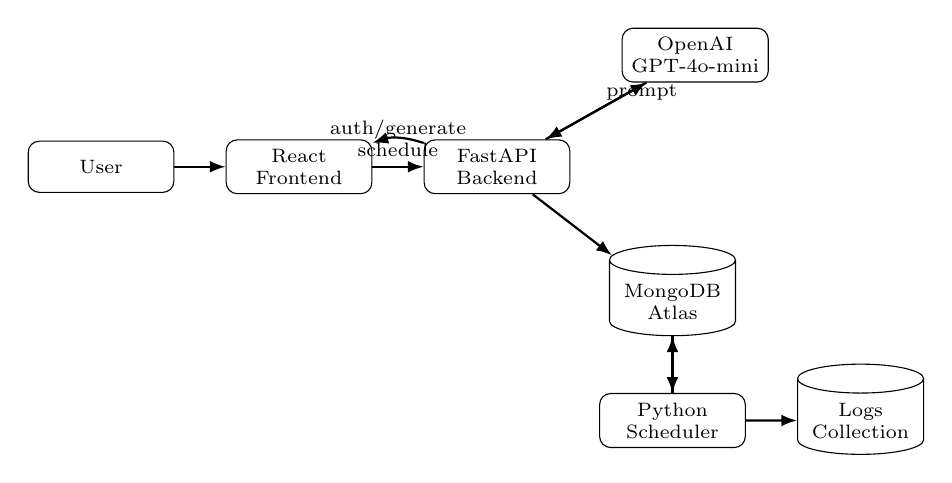
\begin{tikzpicture}[
    node distance=0.72cm and 0.65cm,
    every node/.style={font=\scriptsize},
    box/.style={draw, rounded corners, align=center, minimum width=1.85cm, minimum height=0.65cm},
    db/.style={draw, cylinder, shape border rotate=90, aspect=0.25, align=center, minimum height=0.8cm, minimum width=1.6cm},
    arrow/.style={-{Latex[length=2mm]}, thick}
]
\node[box] (user) {User};
\node[box, right=of user] (react) {React\\Frontend};
\node[box, right=of react] (api) {FastAPI\\Backend};
\node[box, above right=of api] (llm) {OpenAI\\GPT-4o-mini};
\node[db, below right=of api] (mongo) {MongoDB\\Atlas};
\node[box, below=of mongo] (worker) {Python\\Scheduler};
\node[db, right=of worker] (logs) {Logs\\Collection};

\draw[arrow] (user) -- (react);
\draw[arrow] (react) -- node[above, align=center] {auth/generate\\schedule} (api);
\draw[arrow] (api) -- node[above right] {prompt} (llm);
\draw[arrow] (llm) -- (api);
\draw[arrow] (api) -- (mongo);
\draw[arrow] (mongo) -- (worker);
\draw[arrow] (worker) -- (mongo);
\draw[arrow] (worker) -- (logs);
\draw[arrow] (api) to[bend right=18] (react);
\end{tikzpicture}
\caption{High-level architecture of the AI social media automation agent.}
\label{fig:architecture}
\end{figure}

\subsection{Main Workflow}

\begin{figure}[!t]
\centering
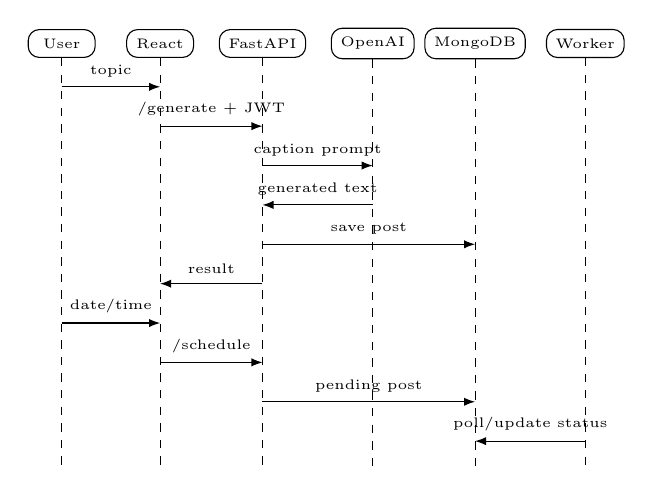
\begin{tikzpicture}[
    every node/.style={font=\tiny},
    actor/.style={draw, rounded corners, align=center, minimum width=0.85cm},
    msg/.style={-{Latex[length=1.4mm]}, thin}
]
\node[actor] (u) at (0,0) {User};
\node[actor] (r) at (1.25,0) {React};
\node[actor] (f) at (2.55,0) {FastAPI};
\node[actor] (o) at (3.95,0) {OpenAI};
\node[actor] (m) at (5.25,0) {MongoDB};
\node[actor] (w) at (6.65,0) {Worker};

\foreach \x in {u,r,f,o,m,w} \draw[dashed] (\x.south) -- ++(0,-5.25);

\draw[msg] (0,-0.55) -- node[above] {topic} (1.25,-0.55);
\draw[msg] (1.25,-1.05) -- node[above] {/generate + JWT} (2.55,-1.05);
\draw[msg] (2.55,-1.55) -- node[above] {caption prompt} (3.95,-1.55);
\draw[msg] (3.95,-2.05) -- node[above] {generated text} (2.55,-2.05);
\draw[msg] (2.55,-2.55) -- node[above] {save post} (5.25,-2.55);
\draw[msg] (2.55,-3.05) -- node[above] {result} (1.25,-3.05);
\draw[msg] (0,-3.55) -- node[above] {date/time} (1.25,-3.55);
\draw[msg] (1.25,-4.05) -- node[above] {/schedule} (2.55,-4.05);
\draw[msg] (2.55,-4.55) -- node[above] {pending post} (5.25,-4.55);
\draw[msg] (6.65,-5.05) -- node[above] {poll/update status} (5.25,-5.05);
\end{tikzpicture}
\caption{Sequence of generation, scheduling, and status update operations.}
\label{fig:workflow}
\end{figure}

\section{Implementation Details}

The backend is implemented in Python using FastAPI and is organized into separate routers for system, authentication, posting, and account-management logic. This modular split is visible in the application's startup file and makes the service easier to extend than a single monolithic endpoint module. Passwords are hashed with bcrypt through Passlib, authenticated routes use JWT bearer tokens, and MongoDB Atlas stores users, generated posts, scheduled items, connected accounts, and worker logs. The frontend is implemented in React and stores the token in browser local storage for session reuse during the prototype stage.

The scheduling worker runs as a separate Python process. It scans the database for pending posts, parses stored date and time fields, and checks whether the scheduled time falls within a narrow execution window. When a LinkedIn platform selection is present, the worker looks up a connected account and calls a publishing service; otherwise it records a simulated result. Success and failure states are both written back to the database, and failures increment retry counters until the post is marked as failed. This behavior is more informative than a simple demo flag because it already captures the operational pattern of queued work, platform resolution, retry handling, and audit logging.

\begin{table}[!t]
\caption{Representative Backend API Endpoints}
\label{tab:api}
\centering
\scriptsize
\begin{tabular}{llll}
\toprule
Endpoint & Method & Protection & Role in workflow\\
\midrule
\texttt{/signup} & POST & No & Create account for a new user\\
\texttt{/login} & POST & No & Return JWT token for later requests\\
\texttt{/generate} & GET & Yes & Request caption and hashtags from the model\\
\texttt{/posts} & GET & Yes & Fetch prior generated posts for one user\\
\texttt{/schedule} & POST & Yes & Store scheduled content as pending work\\
\texttt{/scheduled} & GET & Yes & Fetch scheduled posts and their status\\
\texttt{/testdb} & GET & No & Verify basic database connectivity\\
\bottomrule
\end{tabular}
\end{table}

\begin{table}[!t]
\caption{Main Persistent Collections}
\label{tab:collections}
\centering
\scriptsize
\begin{tabular}{lll}
\toprule
Collection & Main Fields & Practical use\\
\midrule
\texttt{users} & username, password & User identity and hashed credentials\\
\texttt{posts} & topic, result, user, created\_at & Saved AI-generated drafts\\
\texttt{scheduled\_posts} & content, date, time, status & Pending, posted, or failed items\\
\texttt{logs} & action, content/error, time & Worker audit trail and failure history\\
\bottomrule
\end{tabular}
\end{table}

\section{Discussion}

The strongest aspect of the prototype is that it connects generation and scheduling in one place without making the user surrender control. A topic is still chosen by the user, the generated caption is visible before scheduling, and the stored history remains tied to the authenticated account that created it. That sounds simple, but it matters. In many classroom or prototype systems, the language model is the center of the story; here, the surrounding workflow is what makes the tool usable.

Looking at the implementation more closely also makes the limitations very concrete. The `/generate` endpoint is called through a GET request with a topic parameter, generated posts are stored in MongoDB with a username and timestamp, and scheduled items are inserted with a `pending` status until the worker updates them. The worker itself does not publish to a live platform; it only changes state in the database and logs success or failure. That means the current system demonstrates orchestration and traceability of content operations, not real social-platform automation end to end.

There are also some engineering choices that would need revision before serious deployment. The backend currently allows permissive CORS, stores a hardcoded secret key, and includes a direct database connection string in source code. Token storage is handled in browser local storage, which is convenient for a prototype but not ideal from a security perspective. Scheduling also deserves attention because the frontend collects local date and time while the worker compares values in UTC. These are not abstract concerns; they are implementation details visible in the project, and they define the difference between a promising demonstration and a safer production system.

\section{Evaluation Plan}

Because the current repository is a functional prototype, evaluation should combine software testing with a modest content-quality review rather than rely on only one benchmark. At the system level, the most useful tests are straightforward: account creation should reject duplicate usernames, protected endpoints should deny invalid tokens, generated posts should remain isolated by user, and scheduled items should move predictably from pending to posted or failed states. The worker is especially important to test because it is the point where time parsing, retry logic, and platform publishing behavior meet.

Integration testing should follow the actual user flow implemented in the codebase. A realistic scenario would create a user, log in, generate a caption from a topic, schedule that content, and then verify that the worker updates the record and writes a log entry. If a connected LinkedIn account is available, the same evaluation can be extended to observe platform-specific results. If not, the simulation pathway should still be checked to confirm that status changes and audit logging behave correctly.

Content quality is harder to score automatically, so a small rubric-based review is more appropriate. Reviewers can judge whether the generated caption is relevant to the topic, readable, safe for brand use, and useful enough to schedule with minimal edits. A comparison against manual caption writing time would also be informative because the project is intended to reduce drafting effort, not merely produce fluent text. In short, the best evaluation for this system is mixed: partly software reliability, partly human usefulness.

\begin{table}[!t]
\caption{Suggested Prototype Evaluation Metrics}
\label{tab:metrics}
\centering
\scriptsize
\begin{tabular}{lll}
\toprule
Category & Metric & How it can be checked\\
\midrule
Generation quality & Relevance and clarity & Short human rubric\\
Safety & Unsafe or misleading output & Moderation review\\
Reliability & Endpoint and worker success rate & API tests and logs\\
Scheduling accuracy & Due time versus posted time & Worker timestamps\\
Usability & Time to generate and schedule & Small user trial\\
\bottomrule
\end{tabular}
\end{table}

\section{Future Work}

Future work can begin with the parts that are already hinted at in the code. Since a LinkedIn publishing path exists, the next sensible step is to harden connected-account handling and extend the same pattern to additional social platforms rather than rebuild scheduling from scratch. Polling can later be replaced by a queue-based scheduler, but before that, timezone handling and idempotent execution deserve attention because they affect correctness even at small scale.

On the content side, personalization is the most obvious opportunity. The current workflow is topic driven, which keeps the interface simple, but it also limits brand adaptation. Storing preferences for tone, audience, platform, campaign type, and preferred call-to-action would make the generated drafts more useful without changing the overall architecture. A retrieval-based layer could also ground outputs in campaign briefs, product details, or prior approved posts.

There is also room for more responsible automation. Pre-publication moderation, sentiment checks, rate limiting, refresh-token support, stricter CORS, and environment-based secret management would all improve deployment readiness. Finally, a richer analytics layer could move beyond simple history storage and begin to answer operational questions such as which topics are repeatedly scheduled, which outputs need frequent manual edits, and which posting times appear most effective.

\section{Conclusion}

This paper has presented the project as it actually exists: a working social media automation prototype that joins caption generation, authentication, stored history, and scheduled execution inside one application. Its contribution is practical. The system does not propose a new model or a new theory of content automation. Instead, it shows what happens when widely available model access is combined with ordinary application concerns such as user ownership, saved records, scheduling logic, and background processing. That is precisely the level at which many student projects and early startup tools are built.

One of the clearest lessons from both the codebase and the literature is that generative AI becomes more useful when it is embedded in a controlled workflow rather than presented as an independent decision maker. In this project, the user still chooses the topic, inspects the output, and decides whether and when it should be scheduled. That structure is important because social media content can be fluent without being accurate, appropriate, or strategically sound. The prototype therefore makes the most sense as an assistive system, not as a fully autonomous publisher.

The remaining limitations are concrete and easy to name: secret handling should be improved, CORS should be restricted, scheduling should be made timezone-safe, and live platform integrations should be treated with more robust error handling and testing. None of those issues erase the value of the current implementation. If anything, they help place it honestly on the spectrum between demo and deployable tool. As a case study, the project shows that small-scale GenAI systems are most convincing when their strengths, boundaries, and operational responsibilities are stated plainly.

\begin{thebibliography}{15}

\bibitem{grewal2025}
D. Grewal, C. B. Satornino, T. Davenport, and A. Guha, ``How generative AI is shaping the future of marketing,'' \emph{Journal of the Academy of Marketing Science}, vol. 53, pp. 702--722, 2025, doi: 10.1007/s11747-024-01064-3.

\bibitem{cillo2025}
P. Cillo and G. Rubera, ``Generative AI in innovation and marketing processes: A roadmap of research opportunities,'' \emph{Journal of the Academy of Marketing Science}, vol. 53, pp. 684--701, 2025, doi: 10.1007/s11747-024-01044-7.

\bibitem{krugmann2024}
J. O. Krugmann and J. Hartmann, ``Sentiment Analysis in the Age of Generative AI,'' \emph{Customer Needs and Solutions}, vol. 11, art. no. 3, 2024, doi: 10.1007/s40547-024-00143-4.

\bibitem{chen2024}
J. Chen \emph{et al.}, ``When large language models meet personalization: perspectives of challenges and opportunities,'' \emph{World Wide Web}, vol. 27, art. no. 42, 2024, doi: 10.1007/s11280-024-01276-1.

\bibitem{kumar2024llm}
P. Kumar, ``Large language models (LLMs): survey, technical frameworks, and future challenges,'' \emph{Artificial Intelligence Review}, vol. 57, art. no. 260, 2024, doi: 10.1007/s10462-024-10888-y.

\bibitem{hubert2024}
K. F. Hubert, K. N. Awa, and D. L. Zabelina, ``The current state of artificial intelligence generative language models is more creative than humans on divergent thinking tasks,'' \emph{Scientific Reports}, vol. 14, art. no. 3440, 2024, doi: 10.1038/s41598-024-53303-w.

\bibitem{mcguire2024}
J. McGuire, D. De Cremer, and T. Van de Cruys, ``Establishing the importance of co-creation and self-efficacy in creative collaboration with artificial intelligence,'' \emph{Scientific Reports}, vol. 14, art. no. 18525, 2024, doi: 10.1038/s41598-024-69423-2.

\bibitem{mittelstadt2024}
J. M. Mittelstadt, J. Maier, P. Goerke, F. Zinn, and M. Hermes, ``Large language models can outperform humans in social situational judgments,'' \emph{Scientific Reports}, vol. 14, art. no. 27449, 2024, doi: 10.1038/s41598-024-79048-0.

\bibitem{govindankutty2024}
S. Govindankutty and S. P. Gopalan, ``Epidemic modeling for misinformation spread in digital networks through a social intelligence approach,'' \emph{Scientific Reports}, vol. 14, art. no. 19100, 2024, doi: 10.1038/s41598-024-69657-0.

\bibitem{ren2024}
S. Ren \emph{et al.}, ``Reconciling the contrasting narratives on the environmental impact of large language models,'' \emph{Scientific Reports}, vol. 14, art. no. 26310, 2024, doi: 10.1038/s41598-024-76682-6.

\bibitem{kumar2024emoji}
A. Kumar and D. Jain, ``EmoMBTI-Net: introducing and leveraging a novel emoji dataset for personality profiling with large language models,'' \emph{Social Network Analysis and Mining}, vol. 14, art. no. 234, 2024, doi: 10.1007/s13278-024-01400-z.

\bibitem{franceschelli2025}
G. Franceschelli and M. Musolesi, ``On the creativity of large language models,'' \emph{AI \& Society}, vol. 40, pp. 3785--3795, 2025, doi: 10.1007/s00146-024-02127-3.

\bibitem{kudina2025}
O. Kudina and B. de Boer, ``Large language models, politics, and the functionalization of language,'' \emph{AI and Ethics}, vol. 5, pp. 2367--2379, 2025, doi: 10.1007/s43681-024-00564-w.

\bibitem{ding2024}
M. Ding, S. Dong, and R. Grewal, ``Generative AI and Usage in Marketing Classroom,'' \emph{Customer Needs and Solutions}, vol. 11, art. no. 5, 2024, doi: 10.1007/s40547-024-00145-2.

\bibitem{burgess2026}
R. Burgess, K. Waters, E. Spray, and E. Prieto-Rodriguez, ``Using large language models to complement humans for the coding of social media interactions between science teachers,'' \emph{Discover Education}, vol. 5, art. no. 81, 2026, doi: 10.1007/s44217-025-00868-x.

\end{thebibliography}

\end{document}
